\begin{figure}
\center

\pgfplotsset{width=\textwidth,height=8cm}
\pgfplotsset{every axis/.append style={
thick,
tick style={semithick}}}

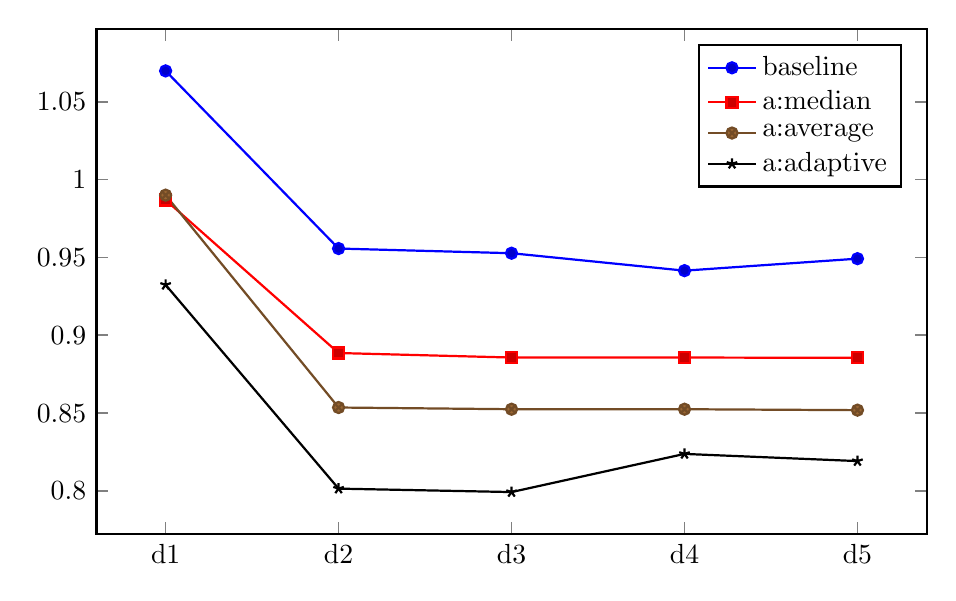
\begin{tikzpicture}

\begin{axis}[
  stack plots=false,
  enlarge x limits=true,
  symbolic x coords={d1,d2,d3,d4,d5},
  xtick=data,
  legend style={
    cells={anchor=west},
    legend pos=north east,
  }
]

\addplot coordinates {
(d1, 1.0698)
(d2, 0.9557)
(d3, 0.9527)
(d4, 0.9415)
(d5, 0.9492)
};
\addlegendentry{baseline}


\addplot coordinates {
(d1, 0.9869)
(d2, 0.8886)
(d3, 0.8857)
(d4, 0.8857)
(d5, 0.8855)
};
\addlegendentry{a:median}
 
\addplot coordinates {
(d1, 0.9900)
(d2, 0.8536)
(d3, 0.8525)
(d4, 0.8525)
(d5, 0.8519)
};
\addlegendentry{a:average}
 
\addplot coordinates {
(d1, 0.9324)
(d2, 0.8015)
(d3, 0.7993)
(d4, 0.8238)
(d5, 0.8192)
};
\addlegendentry{a:adaptive}

\end{axis}
\end{tikzpicture}

\caption[RMSE Variations]{
  RMSE Variations: This plot shows that, while the standard deviation of each method may be high,
  this has more to do with the selected dataset than with their performance in comparison with each other.
  The performance of each of the aggregate methods, as well as the baseline standard method,
  follow similar performance paths across the disjoint datasets.
}
\label{plot:datasets}
\end{figure}




